%! TeX root = ../phd-thesis.tex
%! Author = davidedomini

%----------------------------------------------------------------------------------------
\chapter{Scalable Decentralized Learning}
\label{chap:scalable-rl}
\minitoc
%----------------------------------------------------------------------------------------

\section{Neighbor-Based Strategies for Decentralized Reinforcement Learning}

\subsection{Motivation}
Cooperative \gls{MARL} provides a natural framework for
 systems in which several autonomous agents must learn behaviors that contribute
 to a shared objective.
%
In \gls{CAS}, however, 
 learning must often continue after deployment: 
 agents operate under partial observability, the communication topology may change over time, 
 and the task or environment may evolve in ways that were not represented during offline training.
%
The ability to execute a decentralized policy is therefore not sufficient by itself; 
 the learning process must also remain deployable without relying on
 permanent access to a central coordinator.

As discussed in the background chapters, 
 the dominant cooperative \gls{MARL} paradigm is centralized training with decentralized execution.
%
Centralized access to the agents' observations 
 and experiences reduces the non-stationarity of the learning problem 
 and generally produces more stable and better coordinated
 policies~\cite{DBLP:conf/nips/LoweWTHAM17,DBLP:conf/icml/RashidSWFFW18,DBLP:conf/icml/SonKKHY19}.
%
Nevertheless, 
 this organization introduces a clear separation between an offline training phase 
 and the subsequent deployment of fixed policies.
%
Retraining requires collecting new experience at a central learner, 
 which may be impractical when agents are geographically distributed, intermittently connected,
 or expected to adapt continuously in the field.
%
Moreover, 
 the computation and communication required by centralized training
 become increasingly demanding as the collective grows.

At the opposite end of the spectrum, 
 independent learners update their policies using only locally collected experience~\cite{abed2016comparison}.
%
This organization removes the central bottleneck, 
 scales naturally with the population, 
 and allows training to continue during execution.
%
Its simplicity, however, comes at a substantial cost.
%
From the perspective of each learner, 
 the environment becomes non-stationary because the policies of the other agents change concurrently; 
 local observations also provide only a partial view of the joint task~\cite{DBLP:journals/tcyb/NguyenNN20}.
%
Consequently, 
 independent learning may converge slowly or unstably 
 and lacks an explicit mechanism for coordinating the behaviors learned by different agents.
%
These limitations are especially damaging in cooperative tasks, 
 where individually reasonable actions may still produce a poor collective outcome.

Many real multi-agent systems suggest an intermediate organization between these two extremes.
%
Robots in a swarm, vehicles in a transportation network, 
 and devices in a spatial collective rarely interact with the entire population.
%
Instead, 
 sensing and communication define a time-varying neighborhood around each agent.
% 
Information available within this neighborhood can enrich local training 
 without requiring a global view of the system.
%
Exchanging selected experiences or learned parameters with nearby peers 
 may reduce the instability of independent learning and promote compatible policies, 
 while the bounded scope of the interaction preserves decentralization 
 and limits communication costs.

Neighborhood-based learning has been investigated through consensus 
 and distributed optimization methods, 
 particularly in tabular or actor-critic settings~\cite{kar2012qd,zhang2018fully,DBLP:journals/jmlr/CiosekW20}.
%
Its integration with deep value-based reinforcement learning is less established.
%
In this setting, 
 a central design question is not only \emph{which} agents should communicate, 
 but also \emph{what} they should exchange.
%
Sharing complete neural-network parameters can directly align neighboring policies, 
 but its communication cost grows with model size.
%
Sharing individual experiences is considerably lighter, 
 but influences neighboring policies only indirectly through subsequent training.
%
Selecting a single neighbor, aggregating several neighbors, or disseminating experiences 
 therefore induces different trade-offs among coordination quality,
 stability, and communication overhead.

This section investigates whether these local exchanges can bridge the gap 
 between centralized and fully independent learning.
%
It considers complementary neighbor-based strategies operating on model parameters
 and experience data, and evaluates them against both centralized training 
 and independent decentralized learning.
%
The analysis focuses on three properties: 
 the quality and stability of the learned collective behavior, 
 the ability of the resulting policies to remain effective as the number of agents increases, 
 and the communication cost introduced by local information exchange.
%
The objective is not to reproduce global centralized training through the network,
 but to determine how much of its coordination benefit can emerge from bounded
 peer-to-peer interactions while retaining online adaptation and decentralized control.


\subsection{Formalization}
This section introduces three neighboring-based distributed learning strategies 
 for multi-agent reinforcement learning.
%
These strategies leverage local interactions between agents 
 to improve learning efficiency and coordination.
%
For this investigation, 
 we focus on Deep Q-Learning as the underlying learning algorithm,
 and we consider the following strategies: 
 k-nearest neighbor averaging, k-nearest neighbor consensus, and experience sharing.

\paragraph{K-Nearest Neighbor Definition}
The proposed strategies rely on the concept of k-nearest neighbors.
%
Formally, 
 consider a \emph{weighted} communication graph $\mathcal{G} = (N, E, W)$, 
 where $N$ is the set of agents, 
 where $W: E \rightarrow \mathbb{R}^+$ is a weight function assigning a positive weight to each edge.  
%
Let $d(i,j)$ denote the shortest path length between agents $i$ 
 and $j$ in the weighted graph $\mathcal{G}$. 
%
This can be calculated, 
 for instance, using Dijkstra's algorithm. 
%
The length of a path is the sum of the weights of the edges along the path. 
%
If no path exists between $i$ and $j$, we set $d(i,j) = \infty$.
%
Then, 
 the set of $k$-nearest neighbors of agent $i$ is defined as:
\begin{equation}
  \mathcal{N}_k(i) = \{ j \; \mid \; i \neq j, \; \text{rank}(d(i,j)) \leq k \}
\end{equation}
  where $\text{rank}(d(i,j))$ denotes the rank of the distance $d(i,j)$ among all distances from agent $i$ to other agents in the neighborhood, sorted in ascending order (e.g, $\text{rank}(d(i,j)) = 1$ for the smallest distance).
Ties can be broken arbitrarily.

\paragraph{K-Nearest Neighbor Averaging}
In this strategy, 
 each agent maintains a local Q-network and shares its Q-values with its neighbors.
%
The neighbors average the received Q-values 
 and use the result to update their own Q-networks. 
%
This approach allows agents to learn from their neighbors' experiences, 
 potentially improving learning efficiency and coordination.
%
Formally, 
 giving $\theta^t_i, i \in N$ the parameters of the Q-networks of the agent $i$ at the time $t$,
 the update rule for agent $i$ at time $t+1$ is:
\begin{equation}
  \theta^{t+1}_i = \theta^t_i + \alpha \sum_{j \in \mathcal{N}_k(i)} \frac{1}{k} \theta^t_j
\end{equation}

\paragraph{K-Nearest Neighbor Consensus}
In case of homogeneous agents (i.e., when all agents have the same action and observation space),
%
the goal of learning is to find a common policy that all agents can follow.
%
This approach is typically used in large-scale systems where agents are identical 
 and need to reach a consensus---see~\cite{DBLP:conf/eusipco/BaldazoPZ19}.
%
Instead of directly enforcing a shared policy, 
 we allow each agent to learn independently and periodically select the best-performing agent within its neighborhood as a reference. 
%
This approach facilitates decentralized exploration 
 while promoting consensus towards a high-performing policy.
%
Formally,
 let $R_i(t)^n$ be the average reward obtained by agent $i$ over the last $n$ episodes,
 namely $R_i(t)^n = \frac{1}{n} \sum_{k=t-n}^{t} r_i(k)$.
%
At each time step $t$, 
 each agent $i$ identifies the best-performing neighbor $b_i(t)$ 
 within its $k$-neighborhood $\mathcal{N}_i^k$:
%
$$b_i(t) = \underset{j \in \mathcal{N}_k(i)}{\operatorname{argmax}} \; R_j(t)^n$$
%
Agent $i$ then updates its Q-network parameters $\theta_i$ using the parameters of the best-performing neighbor, 
 namely:
$\theta_i^{t+1} \leftarrow \theta_{b_i(t)}^t$.
%
This process repeats at every consensus update interval.  
%
Choosing an appropriate interval balances independent exploration with consensus convergence.

\paragraph{Experience Sharing}
This approach is typically used in centralized training to improve sample efficiency 
 and learning stability~\cite{marl-book}.
%
In our distributed setting, 
 each agent maintains its own experience replay buffer, 
 but also augments it by collecting a fraction of each neighbor's buffer.
%
This allows agents to learn from each other's experiences, 
 potentially accelerating learning and improving coordination because agents can learn from each other's mistakes 
 and successes.
%
Formally, 
 we define: 
 $\mathcal{D}^t_i$ the replay buffer of the agent $i$ at time $t$,
 $\beta \in \mathbb{N}^+ $ the number of experiences to collect from each neighbor,
 $\phi: \mathcal{D} \times \mathbb{N}^+ \to \mathcal{D}$ a function that, 
 given a replay buffer $H$ and a positive natural number $k$, 
 extracts a subset of cardinality $k$ from $H$.
%
The update rule for agent $i$ at time $t+1$ is:
\begin{equation}
   \mathcal{D}^{t+1}_i = \mathcal{D}^t_i \cup \bigcup_{j \in \mathcal{N}_k(i)} \phi(\mathcal{D}^t_j, \beta)
\end{equation}

\paragraph{Neighboring-Based Training with Deep Q-Learning}
The neighboring-based training strategies can be integrated with Deep Q-Learning 
 to enable distributed learning in multi-agent settings.
%
The algorithm follow the same structure as the Deep Q-Learning algorithm, 
 but with the addition of the neighboring-based interactions.
%
This may happen with a different frequency for each strategy, 
 depending on the communication overhead and the desired level of coordination.
%
In \Cref{alg:neighbor_dqn} we provide a detailed description of the integration 
 of the neighboring-based strategies with Deep Q-Learning.

\begin{algorithm}
    \caption{Neighbor-Based Deep Q-Learning}
    \label{alg:neighbor_dqn}

    \begin{algorithmic}[1]
        \ForAll{agents $i \in N$}
            \State Initialize Q-network
                $Q^i(o^i, a^i; \theta^i)$
            \State Initialize target network
                $Q^{i-}(o^i, a^i; \theta^{i-})$
            \State Initialize replay buffer $\mathcal{D}^i$
        \EndFor

        \For{$episode = 1$ to $M$}
            \ForAll{agents $i \in N$}
                \State Initialize observation $o_0^i$
            \EndFor

            \For{$t = 0$ to $T$}
                \ForAll{agents $i \in N$}
                    \State Select action $a_t^i$ using an
                        $\epsilon$-greedy policy based on
                        $Q^i(o_t^i, a^i; \theta^i)$
                    \State Execute $a_t^i$ and observe
                        $r_{t+1}^i$ and $o_{t+1}^i$
                    \State Store
                        $(o_t^i, a_t^i, r_{t+1}^i, o_{t+1}^i)$
                        in $\mathcal{D}^i$
                    \State Sample a mini-batch from $\mathcal{D}^i$
                    \State Calculate target values using the selected
                        neighbor-based strategy
                    \State Update $\theta^i$ by minimizing the
                        temporal-difference error

                    \If{$t \bmod C = 0$}
                        \State Update the target network:
                            $\theta^{i-} \gets \theta^i$
                    \EndIf

                    \If{$t \bmod S = 0$}
                        \State Perform the selected neighbor-based strategy
                    \EndIf
                \EndFor
            \EndFor
        \EndFor
    \end{algorithmic}
\end{algorithm}

\subsection{Evaluation}
All the experiments and data produced are reproducible 
 and publicly available\footnote{\url{https://github.com/davidedomini/experiments-2024-SAC-marl-neighbouring-strategies}}.

\subsubsection{Simulated environment}
The proposed multi-agent environment is a variant of the ``gather the items'' scenario, 
 designed to study the impact of neighborhood strategies. 
%
It consists of a 2D Euclidean space populated by $A$ agents and $T$ targets, 
 initially placed at random locations.
%
The objective is for the agents to work together to capture all targets, 
 resulting in a successful termination of the environment episode.
%
A maximum time limit of $T_{max} = 300$ time steps is enforced to prevent indefinite 
 episodes---this hyperparameter has nonetheless been chosen to ensure that each episode is long enough for the agents to complete the task.

At each time step $t$, 
 each agent $a$ receives an observation $o_a^t$ composed of the following elements:
\begin{itemize}
  \item \emph{Neighborhood perception}: an agent $a$ perceives the relative positions (distance and direction) 
   of its $A_v$ (paramers of the environment) the nearest neighboring agents. 
   This information is represented as a set $\mathcal{V}_a^t = \{(d_{aj}^t, \theta_{aj}^t) | j \in \text{Nearest } A_v \text{ agents}\}$, 
   where $d_{aj}^t$ is the Euclidean distance between agent $a$ and agent $j$ at time $t$, 
   and $\theta_{aj}^t$ is the angle between the vector pointing from agent $a$ to agent $j$ and a fixed reference axis.
  \item \emph{Target perception}: an agent $a$ perceives the relative positions (distance and direction) 
   of its $T_v$ (parameter of the environment) the nearest targets. 
  This is represented as a set $\mathcal{T}_a^t = \{(d_{ak}^t, \theta_{ak}^t) | k \in \text{Nearest } T_v \text{ targets}\}$, with $d_{ak}^t$ 
   and $\theta_{ak}^t$ defined analogously to the neighborhood perception.
  \item \emph{Memory}: an agent $a$ maintains a memory $\mathcal{H}_a^t$ of past perceptions, 
   storing the neighborhood and target perceptions from the previous $H_t$ time steps. 
  Formally, $\mathcal{H}_a^t = \{\mathcal{N}_a^{t-\tau}, \mathcal{T}_a^{t-\tau} | \tau = 1, \dots, H_t\}$. 
  This can be represented as a tensor of shape $(H_t, A_v + T_v, 2)$, 
   where the last dimension represents the relative distance and angle for each perceived agent or target.
\end{itemize}
The complete observation $o_a^t$ at time $t$ for agent $a$ is thus given by $o_a^t = (\mathcal{N}_a^t, \mathcal{T}_a^t, \mathcal{H}_a^t)$.

Communication between agents is restricted to a neighborhood $\mathcal{C}_a^t \subseteq \mathcal{N}_a^t$ 
 and depends on a communication graph $\mathcal{G}$ that defines the communication links between agents. 
% 
In this work, 
 the graph is based on a k-nearest neighbor topology, 
 where each agent communicates with its $k$ (parameter of the simulation) nearest neighbors.
%
This communication enables the exchange of information such as Q-values or experiences 
 using on of the neighboring-based strategies discussed in \Cref{sec:neighboring}.
%
The action space for each agent is discrete, 
 consisting of eight possible movements corresponding to the cardinal and diagonal directions on a grid.

This environment provides a challenging coordination problem, 
 requiring agents to learn individual target-seeking behaviors and collaborative strategies 
 to minimize retrieval time. 
%
It serves as a suitable testbed for evaluating the effectiveness 
 of neighbor-based decentralized training approaches.

\paragraph{Reward function}

In the proposed environment,
the reward function combines individual objectives,
such as collision avoidance,
with the collective objective of gathering all target items
as quickly as possible.
%
For each agent $a$ at time $t$,
the reward consists of five components.

The collision term penalizes an agent when its action area
intersects that of another agent:
%
\begin{equation}
\psi_t^a =
\begin{cases}
    0, & \text{if no intersections occur}, \\
    -2 \lvert I_a^t \rvert, & \text{otherwise},
\end{cases}
\end{equation}
%
where $I_a^t$ denotes the set of agents whose action areas
intersect that of agent $a$.

A constant time-step penalty $\sigma$,
defined as a hyperparameter,
encourages agents to complete the task in as few steps as possible.

The agent also receives a reward when it moves closer
to one of the visible target items:
%
\begin{equation}
\xi_t^a =
\delta
\max_{i \in V_a^t}
\Bigl(
    d(p_a^t, p_i^t)
    -
    d(p_a^{t+1}, p_i^{t+1})
\Bigr),
\end{equation}
%
where $p_a^t$ and $p_i^t$ denote the positions of agent $a$
and item $i$ at time $t$, respectively,
$V_a^t$ is the set of items visible to the agent,
and $\delta$ is a scalar hyperparameter controlling
the contribution of this term.
%
The difference is positive when the agent approaches an item
and negative when it moves away,
thereby discouraging aimless movement.

Agents are additionally rewarded for increasing their distance
from nearby agents,
encouraging them to spread across the environment
and explore different areas:
%
\begin{equation}
\chi_t^a =
\frac{1}{2\lvert N_a^t\rvert}
\sum_{a_j \in N_a^t}
\Bigl(
    d(p_a^{t+1}, p_{a_j}^{t+1})
    -
    d(p_a^t, p_{a_j}^t)
\Bigr),
\end{equation}
%
where $N_a^t$ denotes the neighborhood of agent $a$
at time $t$.

Finally,
an agent is rewarded whenever a visible item is collected,
regardless of which agent collects it:
%
\begin{equation}
\rho_t^a = 100 \lvert C_a^t \rvert,
\end{equation}
%
where $C_a^t$ is the set of items visible to agent $a$
that are collected at time $t$.
%
Assigning this reward to all agents encourages cooperative behavior,
as each agent benefits from the progress of the team.

The final reward assigned to agent $a$ at time $t$ is:
%
\begin{equation}
r_t^a =
\psi_t^a
-
\sigma
+
\xi_t^a
+
\chi_t^a
+
\rho_t^a.
\end{equation}

\subsection{Experimental setup}
The described environment was implemented using 
 the \emph{Gymnasium} framework~\cite{DBLP:journals/corr/abs-2407-17032}.
%
Moreover, 
 we employed the following libraries to implement the learning algorithms namely: 
 \emph{Ray}~\cite{DBLP:conf/osdi/MoritzNWTLLEYPJ18} 
 (in particular, its module \emph{RLlib}~\cite{DBLP:conf/icml/LiangLNMFGGJS18}),
 and \emph{PyTorch}~\cite{DBLP:conf/nips/PaszkeGMLBCKLGA19}.

We ran a total of $42$ training experiments, namely: 
 $6$ different methods (centralized, distributed, MAPPO and the three neighbor-based strategies discussed).
%
Each method was evaluated across 10 distinct random seeds 
 to enhance the statistical robustness of the observed results.
%
Each experiment consisted of $50$ training episodes. 
%
In these episodes, 
 we fix the number of agents to $4$, $A_v = 3$, $T_v = 3$, $H_t = 3$, $k = 2$, $\sigma = 1$ and $\beta = 1$.
%
As learning algorithms we employed the Deep Q-Learning algorithm and MAPPO.

Furthermore, we ran $15$ evaluation experiments, namely: 
 $5$ different methods and for each method we varied the number of agents ($8$, $16$ and $32$) 
 to assess the metrics under various conditions leaving the other parameters fixed.
% 
In this case, 
 for each experiment we ran $100$ evaluation episodes.

\subsection{Evaluation metrics} 
In our experiments, 
 we employed two metrics to evaluate the performance of the learning agents 
 and monitor the quality of the training process, namely: 
 \begin{enumerate*}[label=(\roman*)]
  \item \emph{Mean Episode Reward} ($R_{mean}$); and
  \item \emph{Mean Episode Length} ($L_{mean}$).
 \end{enumerate*} 

$R_{mean}$ measures the average cumulative reward the agent obtains during each episode, 
  serving as a direct indicator of how well each agent is performing in achieving its task.
%
Formally, 
 for a certain episode $i$, composed of $n$ agents, last $T$ time steps, the total reward $R_i$ is calculated as:
 \[ R_i = \sum_{t=0}^{T} \sum_{j=1}^{n} r^j_t \]
 where $r^j_t$ is the reward obtained by agent $j$ at time step $t$. 
%
The reward $R_{mean}$, 
 for the all the episodes N, 
 can be calculated as the arithmetic mean of the individual rewards per episode $R_i$.

On the other hand, 
 the $L_{mean}$ represents the average number of time steps needed to reaching the terminal state, i.e., no more items to collect. 
%
It provides insights into the agent's efficiency in completing tasks, especially in environments 
 where shorter episodes indicate better performance. 
%
Formally:
 \[ L_{mean} = \frac{1}{N} \sum_{i=1}^{N} L_i \]
 where $L_i$ is length of $i$-th episode.

\begin{figure}
  \centering
  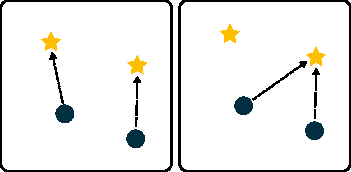
\includegraphics[width=0.4\linewidth]{figures/ch08/sac/behavior.pdf}
  \caption{Examples of cooperative and uncoordinated behavior. 
  (Left) desired, agents effectively choose different paths to collect different items. 
  (Right) undesired, agents cover the same path to collect the same item.}
  \label{fig:behavior}
\end{figure}


\subsection{Results}\label{sec:results}

\paragraph{Performance comparison}
\Cref{fig:results} shows that employing a centralized training (i.e., CTDE) approach allows the model to converge 
 more rapidly--in terms of episodes--to a higher reward compared to a fully decentralized approach (i.e., DTDE). 
%
This difference becomes even more evident when considering the $L_{mean}$, 
 where CTDE not only converges faster but also solves the task using shorter episodes than DTDE. 
 
Additionally, 
 we implemented another state-of-the-art algorithm, namely MAPPO, as a baseline for comparison. 
%
However, 
 MAPPO performed worse than both CTDE and DTDE across both metrics---yielding lower results and exhibiting less stability, 
 as reflected in its higher standard deviation. 

Regarding the proposed neighbor-based approaches, 
 it can be observed that both \emph{experience sharing} and k-NN averaging enhance the performance of DTDE,
 achieving results comparable to CTDE while also increasing learning stability. 
% 
On the other hand, 
 k-NN consensus maintains performance levels similar to DTDE, 
 which may be attributed to the simplicity of the implemented consensus policy. 
%
Nevertheless, 
 it remains more stable and achieves better performance than MAPPO.

\begin{figure*}
  \centering
  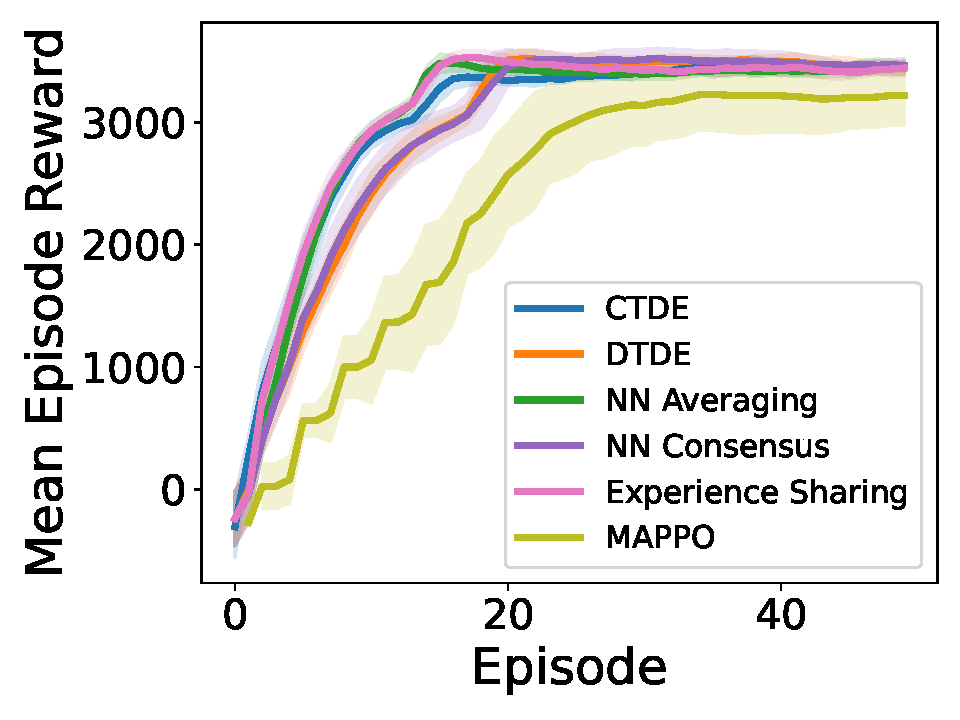
\includegraphics[width=0.4\linewidth]{figures/ch08/sac/episode_reward_mean.pdf}
  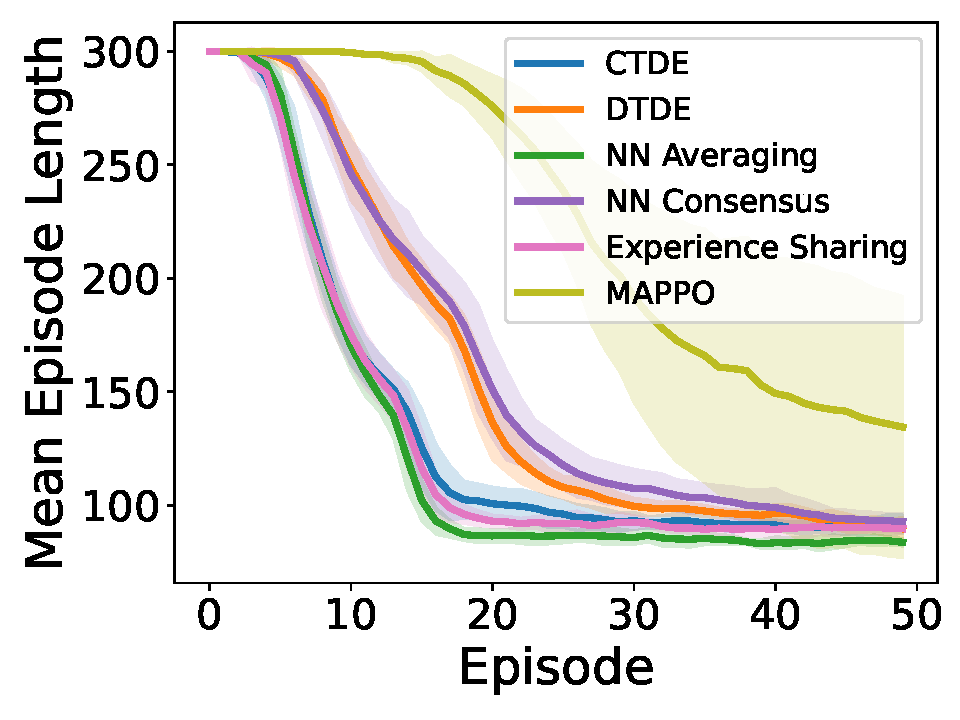
\includegraphics[width=0.4\linewidth]{figures/ch08/sac/episode_len_mean.pdf}
  \caption{Training performance of neighbor-based decentralized training strategies compared to centralized (CTDE) and fully decentralized (DTDE) approaches. 
  }
  \label{fig:results}
\end{figure*}

\paragraph{Scalability}
To evaluate the scalability of the learned policies, 
 we conducted several experiments by increasing the number of agents--specifically to 8, 16, and 32--and measuring the time required 
 to complete the task (i.e., $L_{mean}$). 

\Cref{fig:time-eval} shows that as the number of agents increases, 
 DTDE exhibits both a higher mean time to solve the task and greater instability. 
%
In contrast, CTDE, k-NN averaging, 
 and experience sharing maintain strong performance. 
%
Similar to the training phase, k-NN consensus does not achieve the same results as the other two neighbor-based 
 approaches but remains on par with DTDE in terms of performance.

\begin{figure*}
  \centering
  \begin{subfigure}[b]{0.33\textwidth}
      \centering
      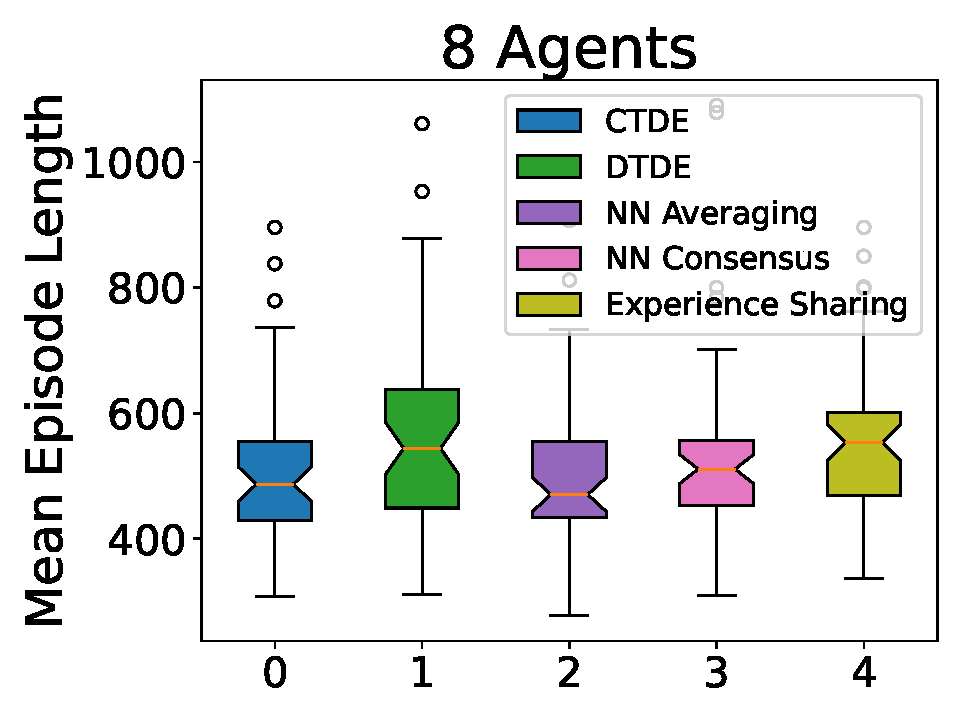
\includegraphics[width=\textwidth]{figures/ch08/sac/mean-time-comparison-8-agents.pdf}
      %\caption{Start of the simulation.}
      % \label{fig:zones1}
  \end{subfigure}
  \begin{subfigure}[b]{0.33\textwidth}
      \centering
      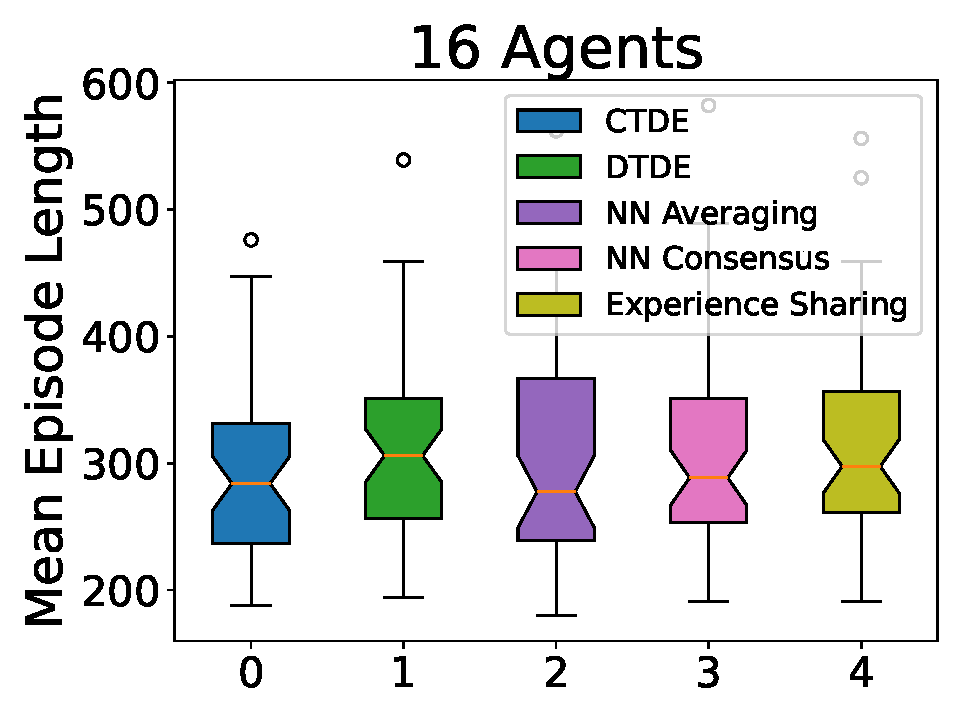
\includegraphics[width=\textwidth]{figures/ch08/sac/mean-time-comparison-16-agents.pdf}
      %\caption{After k time steps of the simulation.}
      % \label{fig:zones2}
  \end{subfigure}
  \begin{subfigure}[b]{0.33\textwidth}
      \centering
      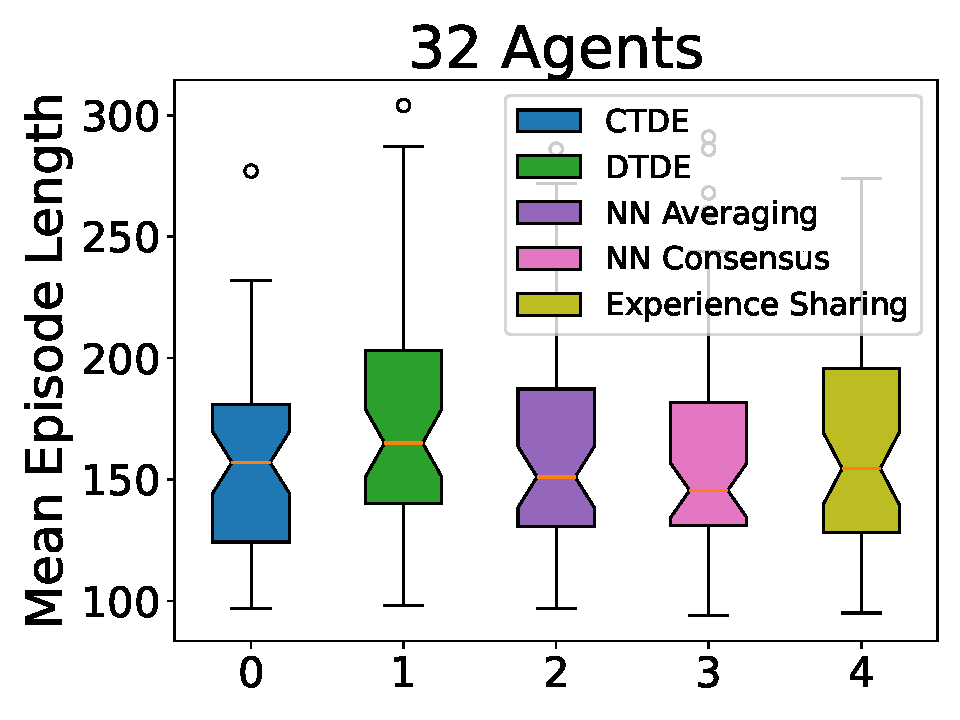
\includegraphics[width=\textwidth]{figures/ch08/sac/mean-time-comparison-32-agents.pdf}
      %\caption{End of the simulation.}
      % \label{fig:zones3}
  \end{subfigure}
  \caption{Scalability comparison of training methods in the evaluation phase.
  DTDE performance degrades with increasing agent numbers, 
  while CTDE and neighbor-based methods maintain comparable efficiency.
  }
  \label{fig:time-eval}
\end{figure*}

\paragraph{Communication overhead}

The proposed neighbor-based approaches, particularly k-NN averaging and experience sharing, 
 achieve performance comparable to CTDE while maintaining a decentralized structure similar to DTDE. 
% 
However, 
 runtime communication is required as agents exchange information with neighbors. 
%
For k-NN consensus, 
 overhead remains constant since each agent communicates with only one neighbor. 
%
In contrast, 
 k-NN averaging and experience sharing scale linearly, though experience sharing's overhead 
 is minimal due to low memory requirements, 
 whereas k-NN averaging incurs higher costs due to larger neural network memory footprints. 
%
All approaches require under 25MB for up to 10 neighbors, 
 making them feasible, with experience sharing 
 being ideal in scenarios with limited communication resources due to its lower overhead.

\begin{figure}
  \centering
  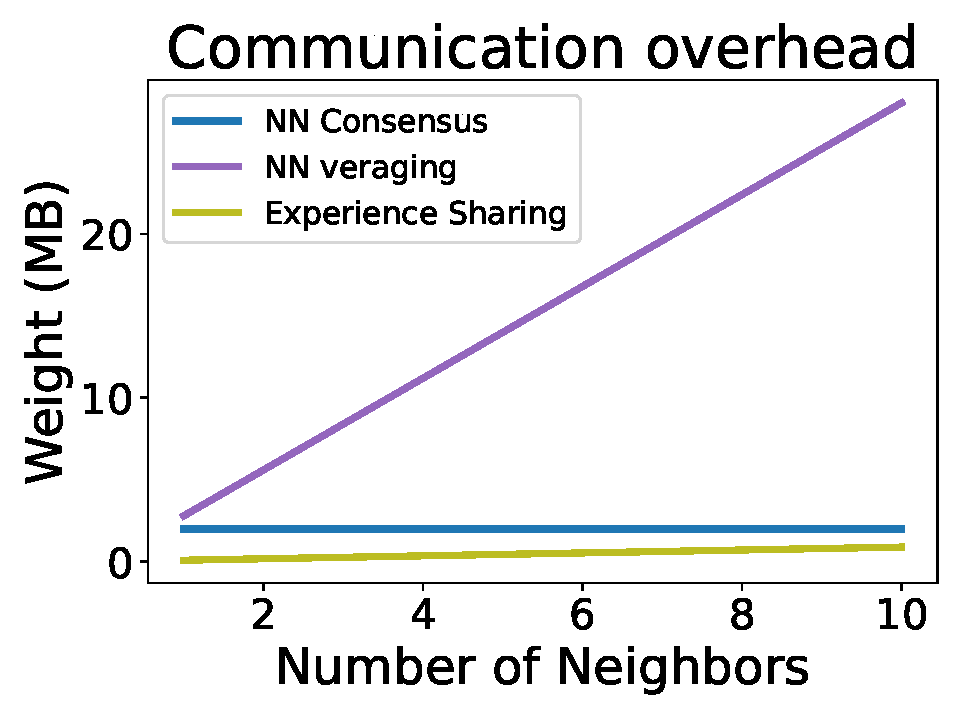
\includegraphics[width=0.5\linewidth]{figures/ch08/sac/scalability.pdf}
  \caption{Communication overhead (in MB) for different neighboring strategies as a function of the number of neighbors.
  }
  \label{fig:scalability}
\end{figure}


%\subsection{Related Works}
\subsection{Future Directions}

\section{Scaling Multi-Agent Reinforcement Learning with GNNs}
\subsection{Motivation}
\subsection{Formalization}
\subsection{Evaluation}
%\subsection{Related Works}
\subsection{Future Directions}